\documentclass{article}
\renewcommand{\thesection}{\Roman{section}}
% \renewcommand{\thesubsection}{\thesection.\Roman{subsection}}
\usepackage{amsmath}
\usepackage{helvet}
\usepackage{graphbox}
\usepackage{subcaption}
\usepackage{blindtext}
\usepackage{parskip}
\usepackage{multicol}
\usepackage{graphicx}
\graphicspath{ {./resources/photos/} }
\setlength{\columnsep}{1cm}
\title{
  % Simulation of misinformation spreading processes
  % in social networks: an application with NetLogo

  Notes
}
\author{Elizer F. Dolorosa}
\date{May 2024}

\begin{document}
\maketitle

\section{CONCEPT}
SBFC Model \textbf{BUT} with the concept of "friend groups" introduced. The idea essentially is that a person's friend group could influence their "SBFC" state.

\begin{figure}[h]
  \begin{subfigure}{0.57\textwidth}
    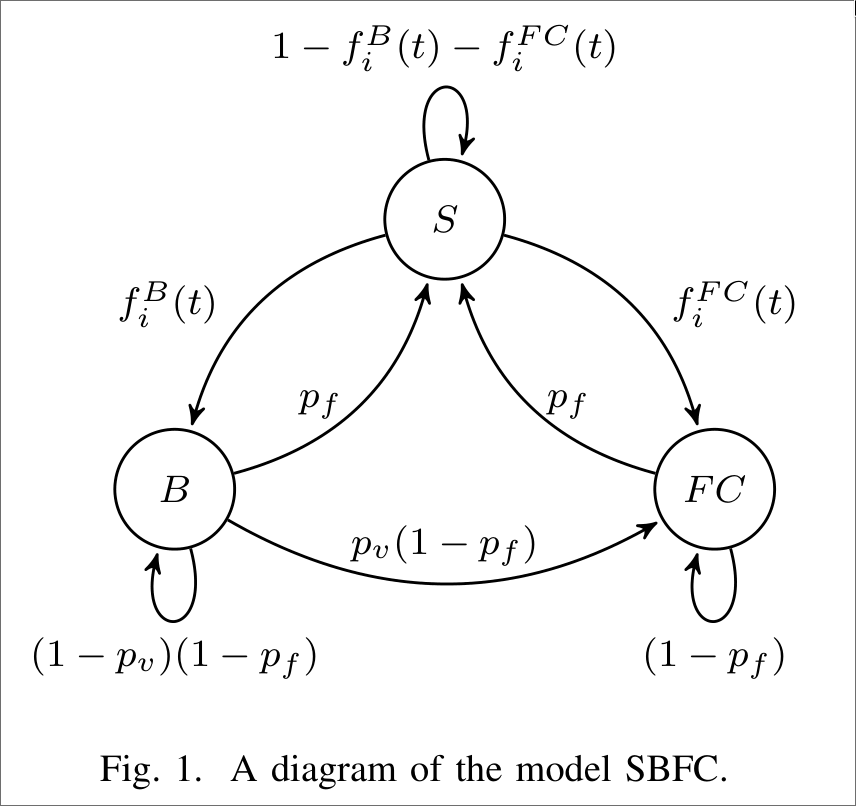
\includegraphics[align=c,width=6.9cm, height=7cm]{sbfc-diagram.png}
  \end{subfigure}
  \begin{subfigure}{0.42\textwidth}
    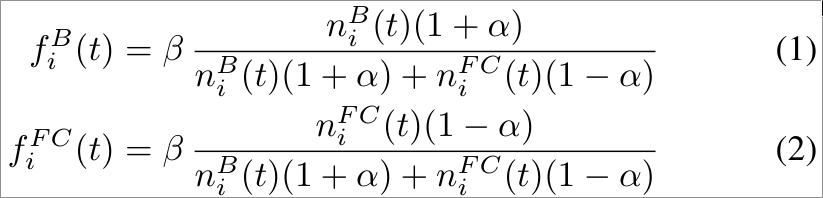
\includegraphics[align=c,width=5cm, height=1.5cm]{transmission-eq.png}
  \end{subfigure}
  % \centering
\end{figure}

Before we begin to assimilate the concept, we assume the following about the new concept:
\begin{enumerate}
  \item The state, and amount of people of friend group stay the same all throughout the simulation
\end{enumerate}

As a result, the following parameters/variables are what I'll add:
\begin{enumerate}
  \item percentage of the population to be in a friend group
  \item percentage of \textit{FC} friend groups
  \item variance of amount of friends in a group [?]
  \item friends' influence
\end{enumerate}

% \pagebreak
Let $h_i^{B|FC}$ return 1 if agent's friend group is $B|FC$ accordingly, otherwise 0.

Let $g_i$ return $i's$ \# of group friends

Let $\omega$ = group friends' influence such that $\omega \in [0,1]$. Thus:

\[g_i^{B|FC} = h_i^{B|FC}g_i(1+\omega)\]

Let $n_i^{B|FC}(t)$ = $B|FC$ neighbors of agent $i$ at time $t$

Therefore we modify $f_i^{B|FC}(t)$ to be:

\[f_i^B(t)=\beta\frac{n_i^B(t)(1+\alpha)+g_i^B}{(n_i^B(t)(1+\alpha)+g_i^B)+(n_i^{FC}(t)(1-\alpha)+g_i^{FC})}\]

\[f_i^{FC}(t)=\beta\frac{n_i^{FC}(t)(1-\alpha)+g_i^{FC}}{(n_i^B(t)(1+\alpha)+g_i^B)+(n_i^{FC}(t)(1-\alpha)+g_i^{FC})}\]

\textit{Verifying} transition should be affected by the
the agent's friend group somehow. We represent this as
the following:

\[ 
  v_g = 
  \begin{cases} 
      1+\omega & \text{if}\ h_i^{FC} = 1 \\
      1-\omega & \text{if}\ h_i^B = 1 \\
      1 & \text{if}\ h_i^{FC} = h_i^B = 0 \\
  \end{cases}
\]
\[ p_v(i) = v_i\;v_g(i) \]

where $v_i$ is the old $p_v$ or the verifying probability

As for \textit{forgetting} transitions, I left it as it is.
% \begin{multicols*}{2}
%
% \section{FIRST SECTION}
% All human things are subject to decay. And when fate summons, Monarchs must obey.
%
% \section{METHODOLOGY}
% All human things are subject to decay. And when fate summons, Monarchs must obey.
%
% \section{RESULTS AND DISCUSSIONS}
% All human things are subject to decay. And when fate summons, Monarchs must obey.
%
% \section{CONCLUSION}
% All human things are subject to decay. And when fate summons, Monarchs must obey.
%
% % \blindtext\blindtext
% \end{multicols*}

\end{document}
